\chapter{Algebraic curves in the projective plane}
\section{Homogenisation of plane curves}
Take an algebraic curve \(y^2=x^2+x^3\) in the affine plane over a field \(k\).
\begin{center}
\documentclass{standalone}
\usepackage{tikz}
\usepackage{pgfplots}
\usepackage{xparse}
\pgfplotsset{compat=1.14}%
\colorlet{curveZero}{gray!85}
\colorlet{curveOne}{blue!60}
\definecolor{curveOneColor}{rgb}{.6,0,0}
\colorlet{curveTwo}{brown!50!gray}
\colorlet{curveThree}{green!40!gray}
\colorlet{curveFour}{red!50!gray}
\NewDocumentCommand\DrawDotInPlot{O{}mmO{}}%
{%
\fill[gray!15,draw=gray] (axis cs:{#2},{#3}) circle [radius=1.6pt] node[above,black,#4] {\(#1\)};%
}%
\NewDocumentCommand\DrawDot{O{}mmO{}}%
{%
\fill[gray!20,draw=gray] ({#2},{#3}) circle (1.6pt) node[above,black,#4] {\(#1\)};%
}%
\NewDocumentCommand\DrawNode{O{}m}%
{%
\fill[gray!20,draw=gray] (#2) circle (1.6pt) node[above,black] {\(#1\)};%
}%
\NewDocumentCommand\DrawDotThreeD{O{}mmmO{}}%
{%
\fill[gray!20,draw=gray] ({#2},{#3},{#4}) circle (1.6pt) node[above,black,#5] {\(#1\)};%
}%
\colorlet{axisColor}{gray!50}
\tikzstyle{shapeZero}=[fill=curveZero,opacity=.4]
\tikzstyle{shapeOne}=[fill=curveOne,opacity=.4]
\tikzstyle{shapeTwo}=[fill=curveTwo,opacity=.4]
\tikzstyle{shapeThree}=[fill=curveThree,opacity=.4]
\tikzstyle{groupElementLabel}=[minimum size=2.4em]
\tikzstyle{groupElement}=[minimum size=2.4em,shapeZero,draw=curveZero]
\tikzstyle{cosetOne}=[minimum size=2.4em,shapeOne,draw=curveOne]
\tikzstyle{cosetTwo}=[minimum size=2.4em,shapeTwo,draw=curveTwo]


\begin{document}

\begin{tikzpicture}
\begin{axis}[hide axis,xmin=-2,xmax=2,ymin=-2,ymax=2,width=4cm]
  \addplot[very thick,domain=-1:0,curveZero,samples=200]{sqrt(x^2+x^3)};%
  \addplot[very thick,domain=-1:0,curveZero,samples=200]{-sqrt(x^2+x^3)};%
  \addplot[very thick,domain=0:1,curveZero]{sqrt(x^2+x^3)};%
  \addplot[very thick,domain=0:1,curveZero]{-sqrt(x^2+x^3)};%
\end{axis}
\end{tikzpicture}
\end{document}

\end{center}
The \emph{cone}\define{cone} on the curve is the surface in \(k^3\) given by \(y^2z = x^2z + x^3\).
\begin{center}
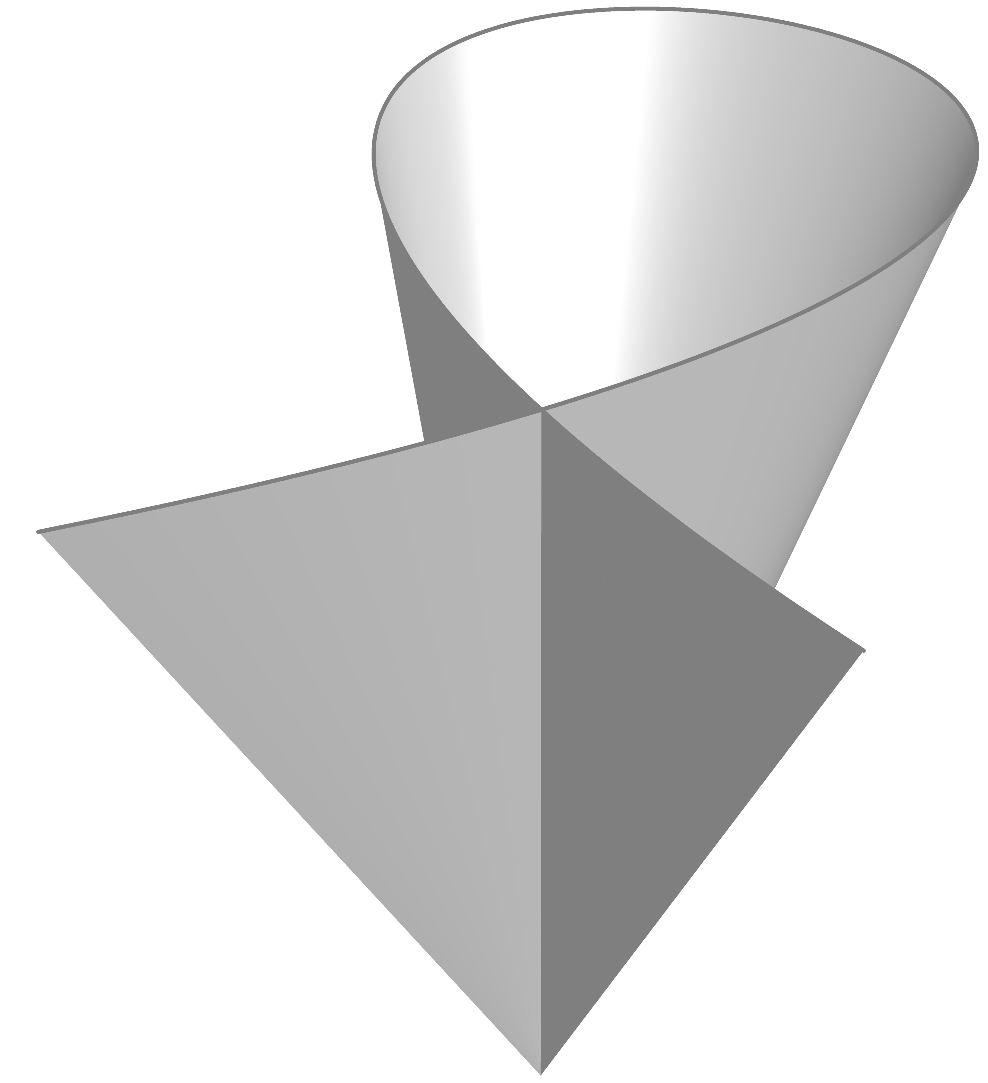
\includegraphics[width=4cm]{cone-over-cubic}
\end{center}
The recipe: given an algebraic equation, like \(y^2=x^2+x^3\):
\begin{enumerate}
\item 
Find the degree \(n\) of the highest term; in this example \(n=3\). 
\item
Invent a new variable \(z\).
\item
Multiply each term by a power of \(z\) so that the total degree of each term reaches \(n\).
\end{enumerate}
A polynomial is \emph{homogeneous}\define{homogeneous!polynomial}\define{polynomial!homogeneous} if all of its terms have the same total degree, i.e. sum of degrees in all variables.
\begin{problem}{projective.plane:homogenise}
Homogenise \(x^2y - x^2 + y = 1 + 2x - y^2x^3\).
\end{problem}
In sage:
\begin{sageblock}
R.<x,y,z> = PolynomialRing(QQ)
p = x^3+x*y+1
p.homogenize(z)
\end{sageblock}
yields \(\sage{p.homogenize(z)}\).

The homogenised polynomial equation \(y^2z = xz^2 + x^3\)  has all terms of degree 3, so if we rescale \(x,y,z\) to \(tx,ty,tz\), we rescale both sides of the equation by \(t^3\), so solutions \((x,y,z)\) rescaled remain solutions \((tx,ty,tz)\).
Thefore every solution lies on a line through the origin consisting of other solutions.
The set of solutions is a surface, which is a union of lines through the origin.
A \emph{projective plane curve}\define{projective!plane curve}\define{plane curve!projective}\define{curve!projective plane} is the set of lines through the origin satisfying a nonzero homogeneous polynomial.

\section{Conics}
\begin{example}
Take a hyperbola \(xy=1\) in the affine plane, 
\begin{center}
\documentclass[tikz]{standalone}
\usepackage{pgfplots}\pgfplotsset{compat=1.12}
\begin{document}
\pgfplotsset{every axis/.append style={
                    axis x line=middle,    % put the x axis in the middle
                    axis y line=middle,    % put the y axis in the middle
                    axis line style={<->,color=blue}, % arrows on the axis
                    xlabel={$x$},          % default put x on x-axis
                    ylabel={$y$},          % default put y on y-axis
            }}
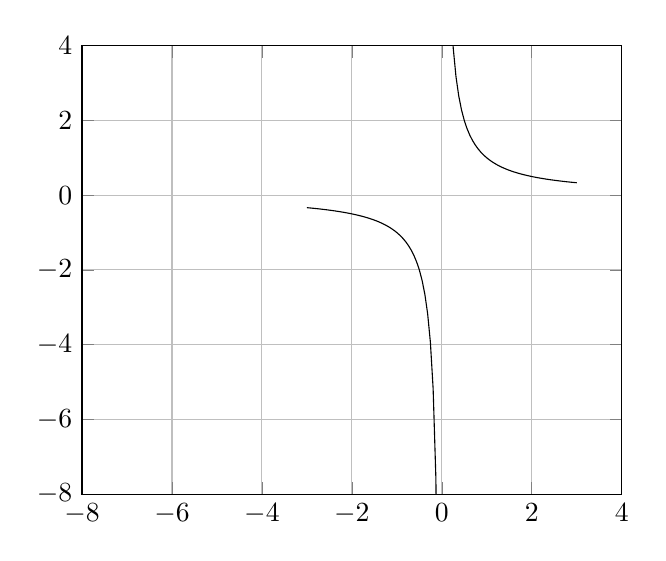
\begin{tikzpicture}
    \begin{axis}[
            xmin=-8,xmax=4,
            ymin=-8,ymax=4,
            grid=both,
            ]
            \addplot [domain=-3:-0.01,samples=50]({x},{1/x}); 
            \addplot [domain=0.01:3,samples=50]({x},{1/x}); 
    \end{axis} 
\end{tikzpicture}
\end{document}

\end{center}
and homogenise to \(xy=z^2\), as we see from three different perspectives:
\begin{center}
\includegraphicsinexample[width=8cm]{cone-over-hyperbola-p0}
\includegraphicsinexample[width=8cm]{cone-over-hyperbola-p1}
\includegraphicsinexample[width=8cm]{cone-over-hyperbola-p2}
\end{center}
If we slice the surface along a plane like \(z=2\), parallel to the plane we drew but higher up, that plane \(z=2\) intersects our surface in a dilated hyperbola.
But if we slice the surface along the plane \(x=1\), we get \(xy=z^2\) to become \(y=z^2\), a parabola:
\includegraphicsinexample[width=8cm]{cone-over-parabola}
Suitable linear changes of variable interchange the \(x\) and \(z\) axes, so suitable projective automorphisms identify the two affine curves: the hyperbola and the parabola.
In particular, the two curves have isomorphic fields of rational functions.
They \emph{don't} have isomorphic rings of regular functions.

If instead we slice our surface with the plane \(x+y=1\),
\includegraphicsinexample[width=8cm]{cone-over-ellipse}
we get \(y=1-x\) plugged in to \(xy=z^2\), which simplifies to 
\[
\pr{x-\frac{1}{2}}^2 + z^2 = \frac{1}{4},
\]
a circle of radius \(\frac{1}{2}\).
So again the circle is birational to the parabola and to the hyperbola, and they all have the same rational function fields.
In these pictures we can see why the conics are called \emph{conics}: they are all slices of the same cone.
\end{example}
\begin{example}
The affine curve \(x^2+y^2=-1\) has no real points on it, but has complex points.
It homogenises to \(x^2+y^2+z^2=0\), a ``sphere of zero radius'', with the origin as its only real point, but with again many complex points.
The complex linear change of variables \(X=x-iy, Y=x+iy, Z=iz\) gives us \(XY=Z^2\), the same projective curve as before.
So these curves are all birational over the complex numbers, and indeed are all identified by automorphisms of the complex projective plane.
\end{example}
\begin{problem}{projective.plane:dehomogenise}
By the same trick of homogenising and dehomogenising in various variables, draw the same sort of pictures for the circle \(x^2+y^2=1\) to see what cone it homogenises to, and what curves it makes when you intersect that cone with the planes (a) \(x=1\), (b) \(y=1\) and (c) \(z=y+1\). 
\end{problem}

\section{Counting intersections of curves}
\epigraph[author={Chico Marx}]{Who are you going to believe, me or your own eyes?}\SubIndex{Marx, Chico}
\begin{example}
A line through a cubic curve
\begin{center}
\inputinexample{cubic-curve-4}
\end{center}
can hit as many as 3 points.
\end{example}
\begin{example}
Two conics
\begin{center}
\newcommand{\conicshift}{-.5}
\inputinexample{2-conics}
\end{center}
can intersect at as many as 4 points, but sometimes only at 3 points:
\begin{center}
\newcommand{\conicshift}{.875}
\inputinexample{2-conics}
\end{center}
\end{example}
\begin{example}
Some conics don't appear to intersect at all
\begin{center}
\newcommand{\conicshift}{4}
\inputinexample{2-conics}
\end{center}
but keep in mind that our points can have coordinates in the algebraic closure, so they actually intersect.
\end{example}
\begin{example}
The conics \(x^2+y^2=1\) and \((x-4)^2+y^2=1\):
\inputinexample{unnested-circles}
intersect at \((x,y)=(2,\pm i \sqrt{15})\). 
\end{example}
\begin{example}
Some conics appear not to have even complex intersections, such as \(x^2+y^2=1\) and \(x^2+y^2=2\).
\inputinexample{nested-circle}
But in the projective plane, we can homogenise to \(x^2+y^2=z^2\) and \(x^2+y^2=2z^2\), and then intersect with the plane \(x=1\), to get \(1+y^2=z^2\) and \(1+y^2=2z^2\), which intersect at \((y,z)=(\pm i,0)\).
\end{example}

\begin{problem}{projective.curves:find.the.points}
Find all points of the curve \(x^3+x^2y+xy^2+y^3+x^2=1\) which lie ``at infinity'', i.e. on the line \(z=0\) in homogeneous coordinates, over the field \(k=\C{}\).
\end{problem}
\begin{answer}{projective.curves:find.the.points}
Homogenize to \(x^3+x^2y+xy^2+y^3+x^2z=z^3\), and then set \(z=0\) to get the homogeneous equation \(x^3+x^2y+xy^2+y^3=0\).
Factor: \((x+y)(x^2+y^2)=0\).
So \(x+y=0\), i.e. \([x,-x,0]=[1,-1,0]\), or \(x^2+y^2=0\), which factors over any field \(k\) which contains an element \(i\) so that \(i^2=-1\), as \((x-iy)(x+iy)=0\), i.e. \(y=\pm ix\), so \([x,ix,0]=[1,i,0]\) and \([x,-ix,0]=[1,-i,0]\).
Hence the points of our curve that lie on the line at infinity are \([1,-1,0], [1,i,0], [1,-i,0]\).
\end{answer}

\begin{problem}{projective.curves:find.the.points.5}
Find all points of the curve \(y^2+y=x^3+x+1\) on the projective plane over the field \(k=\Z{}/5\Z{}\).
\end{problem}
\begin{answer}{projective.curves:find.the.points.5}
Start with the affine plane.
Remember (from problem~\vref{problem:polynomials:quadratic.formula}) that you can use the quadratic formula:
\[
y=\frac{-1\pm\sqrt{1-4(-x^3-x-1)}}{2}.
\]
Simplify, using \(2^{-1}=3\) and \(4=-1\), to:
\[
y=3(-1\pm\sqrt{-x^3-x})
\]
Note that \(0^2=0, 1^2=1, 2^2=4, 3^2=9=4, 4^2=16=1\), so only \(0,1,4\) have square roots.
\begin{itemize}
\item
\(x=0\): \(-x^3-x=0\), \(y=-3=2\), \([x,y,z]=[0,2,1]\).
\item
\(x=1\): \(-x^3-x=3\), no square root of \(3\), no solution.
\item
\(x=2\): \(-x^3-x=-8-2=0\), \(y=-3=2\), \([x,y,z]=[2,2,1]\).
\item
\(x=3\): \(-x^3-x=-27-3=0\), \(y=-3=2\), \([x,y,z]=[3,2,1]\).
\item
\(x=4\): \(-x^3-x=-68=2\), no square root of \(2\) no solution.
\end{itemize}
We still need the points ``at infinity''.
Homogenize: \(y^2z+yz^2=x^3+xz^2+z^3\), and set \(z=0\): \(0=x^3\), so \(x=0\), i.e. \([x,y,z]=[0,y,0]\), and rescale \(y\) to \([0,1,0]\).
Final answer: \([0,2,1], [2,2,1], [3,2,1], [0,1,0]\).
\end{answer}



\begin{lemma}\label{lemma:finitely.many.lines}
Suppose that \(k\) is an infinite field.
Then for any finite set of lines in \(\Proj[2]{k}\), there are infinitely many points of \(\Proj[2]{k}\) not on any of those lines.
\end{lemma}
\begin{proof}
If we work in the affine plane, the points \((x,y)\) lying on those lines must satisfy one of the associated linear equations, say \(y=m_i x + b_i\) or \(x=c_i\).
Pick a number \(x_0\) not among the constants \(c_i\).
Now we have finitely many values \(y=m_i x_0 + b_i\) to avoid; pick \(y\) to not be one of those.
\end{proof}


\begin{lemma}\label{lemma:one.variable.splits}
Every nonzero homogeneous polynomial of degree \(n\) in two variables over a field \(k\) has \(n\) roots, counted with multiplicities, in \(\Proj[1]{\bar{k}}\), and so splits into a product of homogeneous linear factors over \(\bar{k}\).
\end{lemma}
\begin{proof}
As part of the proof, we define multiplicities of zeroes of a homogeneous polynomial \(p(x,y)\) to be multiplicities of linear factors.
So we are saying precisely that \(p(x,y)\) factors into \(n\) linear factors.
If \(p(x,y)\) has a linear factor, divide it out and apply induction.
Since \(y\) is not a linear factor of \(p(x,y)\), \(p(x,1)\) has degree \(n\), say \(p(x,1)=a(x-x_1)\dots(x-x_n)\).
The homogeneous polynomial
\[
r(x,y) \defeq p(x,y)-a(x-x_1y)(x-x_2y)\dots(x-x_ny)
\]
vanishes at \(y=1\) for any \(x\), so by homogeneity vanishes for any \(y \ne 0\).
Fixing any value of \(x\), there are infinitely many values of \(y\) at which \(0=r(x,y)\), and so \(r(x,y)\) vanishes everywhere.
\end{proof}

\begin{example}
The polynomial 
\[
p(x,y)=x^3+x^2y-2xy^2
\]
becomes 
\[
p(x,1)=x^3+x^2-2x=x(x-1)(x+2),
\]
so that 
\[
p(x,y)=x(x-y)(x+2y).
\]
\end{example}
\begin{example}
The family of curves with \(y^2=ax\) contains the curve \(y^2=0\) when \(a=0\), a line.
So a family of curves of degree \(2\) contains a curve of degree \(1\).
It is natural to think of the curve being a ``double line'' when \(a=0\).
\end{example}

Similarly, we can say that a \emph{multiple component}\define{component!multiple} of a curve means a curve given by an equation which is a positive integer power of an irreducible homogeneous polynomial, say \(0=f(x,y,z)^k\) giving a component with multiplicity \(k\).
From now on, we allow projective plane curves to have components with positive integer multiplicities.





\section{Breaking curves into components}


\begin{theorem}[Study]\define{theorem!Study}\define{Study!theorem}\label{theorem:Study}
Every algebraic curve in the projective plane has a unique decomposition into irreducible algebraic curves, its \emph{components}.
To be more precise, every nonzero homogeneous polynomial in 3 variables \(f(x,y,z)\) has a decomposition
\[
f=a_0 g_1^{k_1} g_2^{k_2} \dots g_n^{k_n},
\]
into a product of a nonzero constant \(a_0\) and several coprime irreducible homogeneous polynomials \(g_j(x,y,z)\) to various positive integer powers, unique up to rescaling the constant and the polynomials by nonzero constants, and writing down the polynomials in perhaps a different order.
\end{theorem}
\begin{proof}
Suppose that \(g\) is an irreducible polynomial and that \(f=0\) at every point in \(\bar{k}\) where \(g=0\). 
We want to prove that \(g\) divides \(f\).
Work in the affine plane \(z=1\).
Think of each equation as a polynomial in one variable \(x\), but with coefficients rational functions of \(y\).
By corollary~\vref{corollary:resultant.effective}, after perhaps a linear change of variables, the resultant in \(y\) vanishes just at those \(x\) values where there are simultaneous roots.
In particular, the number of different values of \(x\) where such roots occur is never more than the degree of the resultant, as a polynomial in \(x\).
For each value \(x=c\) (over \(\bar{k}\)) for which \(g(c,y)\) is not constant, the values of \(y\) at which \(g(c,y)=0\) also satisfy \(f(c,y)=0\), so the resultant vanishes.
Therefore this resultant is the zero polynomial.
If the curve where \(f=0\) is the union of distinct irreducible curves given by equations \(g_i=0\), then each of these \(g_i\) divides \(f\), so their product divides \(f\).
Apply induction on the degree of \(f\).
\end{proof}

\begin{theorem}
Every rational morphism of projective plane algebraic curves \(f \colon B \to C\) is constant or onto a finite union of components of \(C\), at most one for each component of \(B\).
\end{theorem}
\begin{proof}
We can assume that \(B\) is irreducible, and we have already assumed that our field is algebraically closed by definition of the points of the curve.
Our rational morphism is
\[
f(x,y,z)=(p(x,y,z),q(x,y,z),r(x,y,z)).
\]
If \(B=(b(x,y,z)=0)\) then the system of equations
\[
 b(a,b,c)=0, a=a(x,y,z), b=b(x,y,z), c=c(x,y,z)
\]
has (after perhaps a linear change of \(x,y,z\) variables) resultant
eliminating \(x,y,z\) given by some algebraic equation in \(a,b,c\) which specifies which points lie in the image.
By corollary~\vref{corollary:resultant.effective} this equation is not trivial.
Split \(C\) into irreducibles \(C_1, C_2, \dots, C_N\), say \(C_j=\pr{c_j=0}\). 
Then \(c_1 c_2 \cdots c_N \circ f=0\) on \(B\), since \(f\) takes \(B\) to \(C\).
So if \(B=\pr{b(x,y,z)=0}\) then \(b\) is divisible by \(c_1 c_2 \cdots c_N \circ f\) in any affine chart.
If \(c_1 \circ f\) is not zero on \(B\) then divide by it to see that already  \(c_2 \cdots c_N \circ f=0\) on \(B\).
So \(f\) takes \(B\) into \(C_2 \cup \dots \cup C_N\).
We can assume that \(c_j \circ f = 0\) on \(B\) for every \(j\), i.e. that \(B \subset f^{-1}C_j\) for every \(j\), i.e. that 
\[
f(B) \subset \bigcap_j C_j:
\]
there is only one such \(C_j\), i.e. \(C\) is irreducible.
Hence the image is precisely \(C\).
\end{proof}


\section{Counting intersections}

A triangle \(pqr\) is \emph{generic}\define{generic!triangle}\define{triangle!generic} for two algebraic projective plane curves \(B, C\) if 
\begin{enumerate}
\item
neither curve passes through \(q\) and
\item 
no line connecting two intersection points of \(B\) and \(C\) lies through \(q\).
\end{enumerate}
\begin{center}
\documentclass[tikz]{standalone}
\usetikzlibrary{intersections}
\usepackage{xparse}
\colorlet{curveZero}{gray!85}
\colorlet{curveOne}{blue!60}
\definecolor{curveOneColor}{rgb}{.6,0,0}
\colorlet{curveTwo}{brown!50!gray}
\colorlet{curveThree}{green!40!gray}
\colorlet{curveFour}{red!50!gray}
\NewDocumentCommand\DrawDotInPlot{O{}mmO{}}%
{%
\fill[gray!15,draw=gray] (axis cs:{#2},{#3}) circle [radius=1.6pt] node[above,black,#4] {\(#1\)};%
}%
\NewDocumentCommand\DrawDot{O{}mmO{}}%
{%
\fill[gray!20,draw=gray] ({#2},{#3}) circle (1.6pt) node[above,black,#4] {\(#1\)};%
}%
\NewDocumentCommand\DrawNode{O{}m}%
{%
\fill[gray!20,draw=gray] (#2) circle (1.6pt) node[above,black] {\(#1\)};%
}%
\NewDocumentCommand\DrawDotThreeD{O{}mmmO{}}%
{%
\fill[gray!20,draw=gray] ({#2},{#3},{#4}) circle (1.6pt) node[above,black,#5] {\(#1\)};%
}%
\colorlet{axisColor}{gray!50}
\tikzstyle{shapeZero}=[fill=curveZero,opacity=.4]
\tikzstyle{shapeOne}=[fill=curveOne,opacity=.4]
\tikzstyle{shapeTwo}=[fill=curveTwo,opacity=.4]
\tikzstyle{shapeThree}=[fill=curveThree,opacity=.4]
\tikzstyle{groupElementLabel}=[minimum size=2.4em]
\tikzstyle{groupElement}=[minimum size=2.4em,shapeZero,draw=curveZero]
\tikzstyle{cosetOne}=[minimum size=2.4em,shapeOne,draw=curveOne]
\tikzstyle{cosetTwo}=[minimum size=2.4em,shapeTwo,draw=curveTwo]


\begin{document}
\begin{tikzpicture}[scale=3]
\draw[curveZero,very thick] 
({cos(90)},{sin(90)}) node[black,above] {\(q\)} -- 
({cos(90+120)},{sin(90+120)}) node[black,below left] {\(p\)} -- 
({cos(90+2*120)},{sin(90+2*120)}) node[black,below right] {\(r\)} -- cycle;
\draw[curveOne,name path=Bellipse,very thick] ({.5*cos(90)+.5*cos(90+2*120)},{.5*sin(90)+.5*sin(90+2*120)}) arc (30:390:.45);
\draw[curveTwo,name path=Cellipse,very thick] ({.5*cos(90)+.5*cos(90+2*120)},{.5*sin(90)+.5*sin(90+2*120)}) arc (30:390:.3 and .6);
\draw [axisColor, name intersections={of=Bellipse and Cellipse}]
(intersection-1) -- ({cos(90)},{sin(90)}) 
(intersection-2) -- ({cos(90)},{sin(90)}) 
(intersection-3) -- ({cos(90)},{sin(90)}) 
(intersection-4) -- ({cos(90)},{sin(90)}); 
\end{tikzpicture}
\end{document}

\end{center}
A triangle \(pqr\) is \emph{very generic}\define{very generic!triangle}\define{triangle!very generic}
\define{generic!triangle!very} for curves \(B\) and \(C\) if it is generic and there is no intersection point of \(B\) and \(C\) along the line \(qr\).
Keep in mind that we allow intersection points, and points of the triangle, to have coordinates in the algebraic closure of our field.
\begin{center}
\documentclass[tikz]{standalone}
\usetikzlibrary{intersections}
\usepackage{xparse}
\colorlet{curveZero}{gray!85}
\colorlet{curveOne}{blue!60}
\definecolor{curveOneColor}{rgb}{.6,0,0}
\colorlet{curveTwo}{brown!50!gray}
\colorlet{curveThree}{green!40!gray}
\colorlet{curveFour}{red!50!gray}
\NewDocumentCommand\DrawDotInPlot{O{}mmO{}}%
{%
\fill[gray!15,draw=gray] (axis cs:{#2},{#3}) circle [radius=1.6pt] node[above,black,#4] {\(#1\)};%
}%
\NewDocumentCommand\DrawDot{O{}mmO{}}%
{%
\fill[gray!20,draw=gray] ({#2},{#3}) circle (1.6pt) node[above,black,#4] {\(#1\)};%
}%
\NewDocumentCommand\DrawNode{O{}m}%
{%
\fill[gray!20,draw=gray] (#2) circle (1.6pt) node[above,black] {\(#1\)};%
}%
\NewDocumentCommand\DrawDotThreeD{O{}mmmO{}}%
{%
\fill[gray!20,draw=gray] ({#2},{#3},{#4}) circle (1.6pt) node[above,black,#5] {\(#1\)};%
}%
\colorlet{axisColor}{gray!50}
\tikzstyle{shapeZero}=[fill=curveZero,opacity=.4]
\tikzstyle{shapeOne}=[fill=curveOne,opacity=.4]
\tikzstyle{shapeTwo}=[fill=curveTwo,opacity=.4]
\tikzstyle{shapeThree}=[fill=curveThree,opacity=.4]
\tikzstyle{groupElementLabel}=[minimum size=2.4em]
\tikzstyle{groupElement}=[minimum size=2.4em,shapeZero,draw=curveZero]
\tikzstyle{cosetOne}=[minimum size=2.4em,shapeOne,draw=curveOne]
\tikzstyle{cosetTwo}=[minimum size=2.4em,shapeTwo,draw=curveTwo]


\begin{document}
\begin{tikzpicture}[scale=3]
\draw[curveZero,very thick] 
({cos(90)},{sin(90)}) -- 
({cos(90+120)},{sin(90+120)}) -- 
({2*cos(90+2*120)},{sin(90+2*120)}) -- cycle;
\draw[curveOne,very thick,name path=Bellipse] ({.5*cos(90)+.5*cos(90+2*120)},{.5*sin(90)+.5*sin(90+2*120)}) arc (30:390:.45);
\draw[curveTwo,very thick,name path=Cellipse] ({.5*cos(90)+.5*cos(90+2*120)},{.5*sin(90)+.5*sin(90+2*120)}) arc (30:390:.3 and .6);
\draw [axisColor, name intersections={of=Bellipse and Cellipse}]
(intersection-1) -- ({cos(90)},{sin(90)}) 
(intersection-2) -- ({cos(90)},{sin(90)}) 
(intersection-3) -- ({cos(90)},{sin(90)}) 
(intersection-4) -- ({cos(90)},{sin(90)}); 
\end{tikzpicture}
\end{document}

\end{center}

By projective automorphism, we can make any triangle become the one whose vertices are \[[0,0,1],[1,0,0],[0,1,0].\]
This projective automorphism is unique up to rescaling the variables.
In the affine plane, these vertices are the points \((0,0), (\infty,0), (0,\infty)\).
Suppose that our two curves have equations \(B=(b(x,y)=0)\) and \(C=(c(x,y)=0)\).
The triangle is generic just when 
\begin{enumerate}
\item
\((0,\infty)=[0:1:0]\) is not on \(B\) or \(C\), and
\item
no vertical line intersects two intersection points of \(B\) and \(C\).
\end{enumerate}
In a more algebraic description:
\begin{enumerate}
\item
\(b(x,y)\) and \(c(x,y)\) both have nonzero constants in front of their highest terms in \(y\) and
\item
for any constant \(x=x_0\), \(b(x_0,y)\) and \(c(x_0,y)\) have at most one common root in \(y\).
\end{enumerate}
If the triangle is generic, it is also very generic just when there is no zero of the homogeneous polynomials \(b(x,y,z)\), \(c(x,y,z)\) on the line at infinity, i.e. the line \(z=0\), or, in other words, the highest order terms of \(b(x,y)\) and \(c(x,y)\) (which are homogeneous of the same degree as \(b(x,y)\) and \(c(x,y)\)) have no common root on \(\Proj{1}\).
The resultant \(\resultant{b}{c}(x)\) in \(y\) depends, up to constant factor, only on the choice of curves \(B\) and \(C\) and the choice of triangle.
The \emph{intersection number}\define{intersection number} of \(B\) and \(C\) at a point \(p=(x,y)\), denoted 
\(\multiplicity{p}{B}{C}\),\Notation{BCp}{\multiplicity{p}{B}{C}}{multiplicity of intersection of curves \(B\) and \(C\) at point \(p\)} is the multiplicity of \(x\) as a zero of \(\resultant{b}{c}(x)\).
If \(p\) is not a point of both \(B\) and \(C\) then define
\(\multiplicity{p}{B}{C}\defeq 0\).
If \(p\) lies on a common component of \(B\) and \(C\) then let \(\multiplicity{p}{B}{C}\defeq\infty\).
Danger: so far, the intersection number depends on the choice of triangle.
Let \(\intersectionnumber{B}{C}\defeq \sum_p \multiplicity{p}{B}{C}\)\Notation{\#BC}{\intersectionnumber{B}{C}}{total multiplicity of intersection of curves \(B\) and \(C\)} summed over all points \(p\).

\begin{example}
Let \(b(x,y)\defeq y+x\) and \(c(x,y)\defeq y\). 
The intersection points of the lines \((b(x,y)=0)\) and \((c(x,y=0)\) in the affine plane are at \(0=y=y+x\), i.e. at the origin.
In the projective plane, there is no further intersection point, as the equations are already homogeneous.
So the standard triangle is very generic for these two lines.
The resultant of \(b(x,y), c(x,y)\) in \(y\) is \(r(x)=x\).
So the two lines \(B=(y+x=0)\) and \(C=(y=0)\) have \(\multiplicity{(0,0)}{B}{C}=1\).
Similarly any two lines have intersection number 1 at their intersection point.
\end{example}
\begin{example}
Let \(B\defeq (xy^2+y=0)\) and \(C\defeq (xy^2+y+1=0)\).
The curves intersect in the affine plane at 
\[
(x,y)=\pr{-2,-\frac{1}{2}}
\]
(assuming that \(2 \ne 0\) in our field).
Homogenize to find also the intersection point \((0,\infty)=[0:1:0]\).
So the coordinate triangle is not generic.
As previously, if we change \(x\) to \(x+\lambda\) for any constant \(\lambda \ne 0\), our curves change to
\[
B=(\lambda y^3+xy^2+y=0), C=(2\lambda y^3+2xy^2+y+1).
\]
They now intersect at
\[
(x,y)=(-1-\lambda,1)=[-1-\lambda,1,1].
\]
(We previously saw this from looking at the resultant \(r(x)=-\lambda^2(\lambda+1+x)\).)
After homogenizing and then setting \(y=1\), we also find another intersection at \([x,y,z]=[-\lambda,1,0]\).
The standard triangle is generic for these curves, since the two intersection points lie on different lines through \([0,1,0]\).
But it is not very generic, because our second intersection point lies outside the affine plane, on the line at infinity.
We can only calculate the intersection number at the first point, where the resultant vanishes to degree \(1\), so an intersection number
\[
\multiplicity{(-\lambda-1,1)}{B}{C}=1.
\]
The other point is not in the affine plane, so intersection multiplicity is not defined at that point, at least by our definition.
\end{example}

\begin{theorem}[B\'ezout]\label{theorem:baby.B\'ezout}\define{theorem!B\'ezout}\define{B\'ezout!theorem}
Over any field, take two projective algebraic plane curves \(B\) and \(C\) not sharing a common component.
Over some finite degree extension of the field there is a very generic triangle for the curves.
For any generic triangle, \(\intersectionnumber{B}{C} \le \degree{B}\degree{C}\).
A generic triangle is very generic just when equality holds.
\end{theorem}
\begin{proof}
Split \(B\) and \(C\) into irreducibles and add up intersections by multiplying resultants: without loss of generality we can assume that \(B\) and \(C\) are irreducible.

By proposition~\vref{proposition:resultant.degree}, there are at most \(\degree{B}\degree{C}\) values of \(x\) that occur on intersection points, and by the same reasoning at most that number of \(y\) values, so finitely many intersection points.

Since there are finitely many intersection points, there are finitely many lines through them. 
By lemma~\vref{lemma:finitely.many.lines} we can pick one vertex of our triangle to avoid lying on any of them (after perhaps replacing by an extension field), while arbitrarily picking the other two vertices to be any two distinct points.
So we have a generic triangle, and we can assume that its vertices are \((0,0)\), \((\infty,0)\) and \((0,\infty)\).
We can then move the line at infinity to avoid the intersection points (again in some extension field), so there is a very generic triangle.

Pick any generic triangle.
No two intersection points lie on any line through \((0,\infty)\), i.e. on any vertical line: all of the intersection points have distinct \(x\) values.
There is no intersection point at \((0,\infty)\), i.e. the highest order terms in \(y\) in the equations have no common zero.
Therefore even when \(b(a,y)\) drops degree at some value of \(x=a\), \(c(a,y)\) doesn't, so the resultant is the product of the values of \(b(a,y)\) at the roots \(y\) of \(c(a,y)\), vanishing precisely at the values of \(x\) where the curves have an intersection.
In the proof of proposition~\vref{proposition:resultant.degree}, we found the degree of the resultant to be at most \(\degree{b}\degree{c}\) and nonzero.
There are at most a number of intersection points given by the degree of the resultant as a polynomial.
Hence the sum of the intersection numbers over the intersections in the affine plane is the sum of the degree of root over all roots of the resultant, so at most the degree of the resultant.
Our triangle is very generic just when this sum covers all intersection points, as there are none on the line at infinity.

We still need to see that for our very generic triangle, the degree of the resultant is precisely \(\degree{B}\degree{C}\).
The assumption of being very generic is expressed algebraically as saying that the homogeneous polynomials \(b(x,y,z), c(x,y,z)\) have no common roots along \(z=0\).
In other words, \(b(x,y,0)\) and \(c(x,y,0)\) have no common roots on \(\Proj{1}\).
So the resultant of \(b(x,y,0),c(x,y,0)\) in \(y\) is nonzero, and has degree \(\degree{B}\degree{C}\).
But the degree of resultant of \(b(x,y,z), c(x,y,z)\) can be no less for variable \(z\) as for the fixed value \(z=0\).
Therefore the resultant has the required degree.
\end{proof}



\begin{theorem}\label{theorem:intersection.number.definition}
To any two projective algebraic plane curves \(B\) and \(C\) over a field \(k\) and any point \(p\) of the projective plane defined over the algebraic closure \(\bar{k}\) of \(k\), there is a unique quantity \(\multiplicity{p}{B}{C}\) so that
\begin{enumerate}
\item\label{item:B\'ezout.first}
\(\multiplicity{p}{B}{C} = \multiplicity{p}{C}{B}\) and
\item
\(\multiplicity{p}{B}{C}=0\) just when \(p\) does not lie on any common point of \(B\) and \(C\) defined over \(\bar{k}\) and
\item
\(\multiplicity{p}{B}{C}=\infty\) just when \(p\) lies on a common component of \(B\) and \(C\) defined over \(\bar{k}\) and
\item
\(\multiplicity{p}{B}{C}\) is a positive integer otherwise and
\item
two distinct lines meet with intersection multiplicity 1 at their unique point of intersection and
\item
if \(B\) splits into components (perhaps with multiplicities) \(B_1\) and \(B_2\), then \(\multiplicity{p}{B}{C}=\multiplicity{p}{B_1}{C}+\multiplicity{p}{B_2}{C}\) and
\item\label{item:B\'ezout.last}
if \(B\) and \(C\) are defined by homogeneous polynomials \(b(x,y,z)\) and \(c(x,y,z)\) and \(E\) is the curve defined by \(bh+c\) where \(h(x,y,z)\) has degree \(\degree{h}=\degree{b}-\degree{c}\), then \(\multiplicity{p}{B}{C}=\multiplicity{p}{B}{E}\).
\end{enumerate}
Moreover, \(\multiplicity{p}{B}{C}\) can be computed as defined above using any generic triangle.
\end{theorem}
\begin{proof}
In this proof, we write \(\multiplicity{p}{b}{c}\) instead of \(\multiplicity{p}{B}{C}\) if \(B\) is cut out by the equation \(0=b(x,y,z)\) and \(C\) by \(0=c(x,y,z)\).
First we prove that the conditions \ref{item:B\'ezout.first}--\ref{item:B\'ezout.last} determine the multiplicity uniquely.
Since they are independent of choice of affine chart, this ensures that the multiplicity is also independent.
We then check that our definition above satisfies these, so must be determined by these conditions independent of the choice of affine chart made in the definition above.

Any two notions of multiplicity agree on common components of \(B\) and \(C\), and on points not belonging to \(B\) or \(C\), by the conditions above.
So we only need to check points of positive finite multiplicity.
We can assume by induction that \(B\) and \(C\) are both irreducible, and cut out by irreducible homogeneous polynomials \(b\) and \(c\).
Suppose that we have two different methods of calculating an intersection number satisfying our various conditions, one of which we can take to be the definition by the resultant above.
By induction suppose that they agree wherever they both assign a value less than the larger of the two values that they assign as \(\multiplicity{p}{b}{c}\).

Take affine coordinates in which \(p=(0,0)\).
If \(\degree{b}(x,0)=0\) then \(b(x,0)=0\) so \(b(x,y)\) is divisible by \(y\), not irreducible, so our result holds by induction.
The same holds if \(\degree{c}(x,0)=0\).
So both \(b\) and \(c\) have positive degree in each of \(x\) and \(y\) when the other variable is set to zero.
Rescale to get both to have unit coefficient in \(x\):
\begin{align*}
b(x,y) &= x^{\beta} + \dots , \\
c(x,y) &= x^{\gamma} + \dots.
\end{align*}
Suppose (after perhaps swapping the names of \(b\) and \(c\)) that \(\beta \le \gamma\) and let
\[
h(x,y)
\defeq 
c(x,y)-x^{\gamma-\beta}b(x,y).
\]
By construction, \(h(x,0)\) has degree in \(x\) at most \(\gamma-1\).
Our last property of intersection multiplicity above demands that \(\multiplicity{p}{b}{c}=\multiplicity{p}{b}{h}\).
Therefore we can replace \(c\) by \(h\) and repeat, lowering the degree in \(x\) by induction.
This proves uniqueness of intersection multiplicities satisfying our axioms.

We want to prove existence, i.e. that the recipe we defined above satisfies our axioms above.
\begin{enumerate}
\item
Resultants change sign when we swap polynomials, so \(\resultant{b}{c}=-\resultant{c}{b}\).
\item
Follows from theorem~\vref{theorem:baby.B\'ezout}.
\item
Follows from theorem~\vref{theorem:baby.B\'ezout}.
\item
Follows from theorem~\vref{theorem:baby.B\'ezout}.
\item
Follows by direct computation of the resultant.
\item
Follows from lemma~\vref{lemma:resultants.multiply}. 
\item
Follows from proposition~\vref{proposition:factored.resultants}, and the existence of splitting fields.
\end{enumerate}
\end{proof}

We restate B\'ezout's theorem without reference to generic triangles, since the previous theorem proves that they are irrelevant.
\begin{theorem}
[B\'ezout]\label{theorem:B\'ezout}\define{theorem!B\'ezout}\define{B\'ezout!theorem}
Over any field \(k\), take two projective algebraic plane curves \(B\) and \(C\) not sharing a common component.
Over the algebraic closure \(\bar{k}\) of the field, the intersection numbers of the intersection points sum to
\[
\sum_p \multiplicity{p}{B}{C} = \degree{B}\degree{C}.
\]
\end{theorem}


\section{Sage}

Pieter Belmans wrote the following sage code to find the intersection number of two algebraic curves at a point.
First we find the minimum degree of any term in a polynomial \(f(x)\) of one variable.
\begin{sageblock}
def ldegree(f):
    minimum = infinity
    for (n, m) in f.dict():
        minimum = min(minimum, n)
    return minimum
\end{sageblock}
Given any two polynomials \(b, c\) in two variables, we want to figure out what the two variables are:
\begin{sageblock}
def determine_variables(b, c):
    if len(b.variables()) == 2:
        return b.variables()
    if len(c.variables()) == 2:
        return c.variables()
    if len(b.variables()) == len(c.variables()) == 1:
        if b.variables() == c.variables():
            return (b.variable(0), 0)
        else:
            return (c.variable(0), b.variable(0))
    return (0,0)
\end{sageblock}
Finally, we use our definition of intersection number, and induction, to compute intersection numbers recursively.
\begin{sageblock}
def intersection_number(b, c, point = (0,0)):
    (x,y) = determine_variables(b, c)
    # translate both curves to origin and calculate it there
    b = b.subs({x:x + point[0], y:y + point[1]})
    c = c.subs({x:x + point[0], y:y + point[1]})
    # if $b(0,0)\neq 0$ or $c(0,0)\neq 0$ they don't intersect in the origin
    if b.subs({x:0, y:0}) != 0 or c.subs({x:0, y:0}) != 0: 
        return 0
    # if $b$ or $c$ are zero they don't intersect properly
    if b == 0 or c == 0: 
        return Infinity
    # we only look at factors of $x$
    f = b.subs({y:0})
    g = c.subs({y:0})
    # $b$ contains a component $y=0$
    if f == 0:
        # $c$ contains a component $y=0$ too, no proper intersection
        if c == 0: 
            return infinity
        # remove common $y^n$ in $b$, count degree of $x$ in $c$ and recurse
        else:
            f = b.quo_rem(y)[0]
            return ldegree(g) + intersection_number(f, c)
    # $b$ does not contain a component $y=0$
    else:
        # $c$ *does* contain a component $y=0$
        if g == 0:
            g = c.quo_rem(y)[0]
            return ldegree(f) + intersection_number(b, g)
        # we recurse by removing factors of $x$
        else:
            p, q = f.lc(), g.lc()
            r, s = f.degree(), g.degree()
            # we drop the highest degree term
            if r <= s:
                return intersection_number(b, p*c - q*x^(s-r)*b)
            else:
                return intersection_number(q*b - p*x^(r-s)*c, c)
\end{sageblock}
A test run:
\begin{sageblock}
P.<x,y> = PolynomialRing(QQ)
b = P(x^2+y^2)^2+3*x^2*y-y^3
c = P(x^2+y^2)^3-4*x^2*y^2
intersection_number(b,c)
\end{sageblock}
yields \(\sage{intersection_number(b,c)}\), the intersection number at the origin of the curves:
\begin{center}
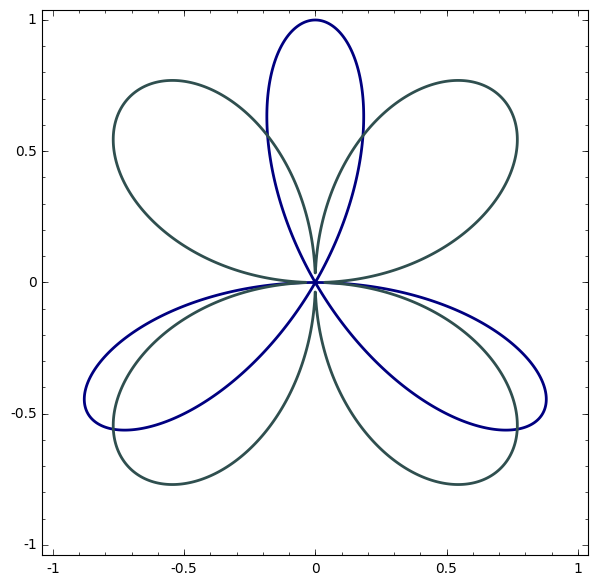
\includegraphics[width=6cm]{curve_intersection}
\end{center}
%p=implicit_plot(b, (x,-1, 1), (y,-1, 1),color="navy",linewidth=2, plot_points=1500)
%q=implicit_plot(c, (x,-1, 1), (y,-1, 1),color="darkslategray",linewidth=2, plot_points=1500)
%show(p+q)
